\documentclass{article}
\usepackage[utf8]{inputenc}

\title{Empowering local IT with open-source tools}
\author{Lauri Võsandi}
\date{January 2015}

\usepackage{natbib}
\usepackage{graphicx}
\usepackage{url}
\usepackage{tikz}

\begin{document}

\maketitle

\section{Introduction}

This minor thesis complements the major thesis
titled \emph{Efficient and Reliable Filesystem Snapshot Distribution}.


\section{Background}

IT is essential infrastructure for every country, especially developing countries.
The harsh reality is that western IT corporations often offer products
and services for developing countries at non-sustainable prices in order
to gain userbase. Once the country has reached certain living standard the
pricing is adjusted accordingly.

As the users have been learning to use particular product,
reluctance to switch is increased due to training costs,
user fustration etc. Most often organizations submit to paying
licensing fees at significantly higher prices due to increased
user discontent.

Starting from the end of 2013 Microsoft does not consider Estonia a
developing country anymore. The implication of the change was that
the Microsoft Windows and Microsoft Office license fees would rise
from current 6 EUR to 60 EUR per month per machine.
According to Ernst \& Young analysis Tallinn could save 490 000 EUR
within 5 years if they would give up Microsoft Office now.
Replacing Windows with Linux would save additional 210 000 EUR.
This was the main motivation for Tallinn Education Department to try
out alternatives. As change from Microsoft Office to LibreOffice was
certain, replacing operating system was more questionable.

In March of 2014 they decided to pilot Linux in 5 educational
institutions: Mustamäe Upper Secondary School [2], Tallinn Mahtra
Primary School [3], Merivälja school [4], Tallinn Mesimummu
kindergarten [5] and Tallinn Tammetõru kindergarten [6].
Procurement competition was won by Arvuti Traumapunkt OÜ [7] and
Silver Püvi hired me to take care of setting up infrastructure servers.
Most of the work so far has been done remotely in conjunction with
local IT-support. Before the migration I had around 7 years of
open-source hacking experience, however I never had experience with
remote management or centralized authentication.


\section{Challenge}

Prior the project I never had experience managing Linux based workstations.
My goal was to provide a platform which would be easier than current Windows
workstations.
In retrospective maintaining Linux-based and in fact
Windows workstations as well concerns several aspects:

\begin{itemize}
\item Provisioning - getting the initial software setup onto the computer
\item Updating - keeping the software up to date
\item Configuration management - adjusting configuration of various software components
\item Central authentication - keeping user accounts off the machines
\item Networked storage - keeping user files off the machines
\end{itemize}

The need for configuration management, central authentication
and networked storage was recognized immideately.


Puppet was chosen for configuration management due to it's
enterprise capabilities and vibrant community.
Foreman was used as Puppet web interface to provide
overview of the inventory.
Initially Puppet was used to also perform software updates, but
it turned out to be a bad idea because even though Ubuntu package
management performs well for most cases, there are still some
corner cases which may render the whole package management
system unusable.

\begin{figure}[!htb]
\centering
\scalebox{0.5}{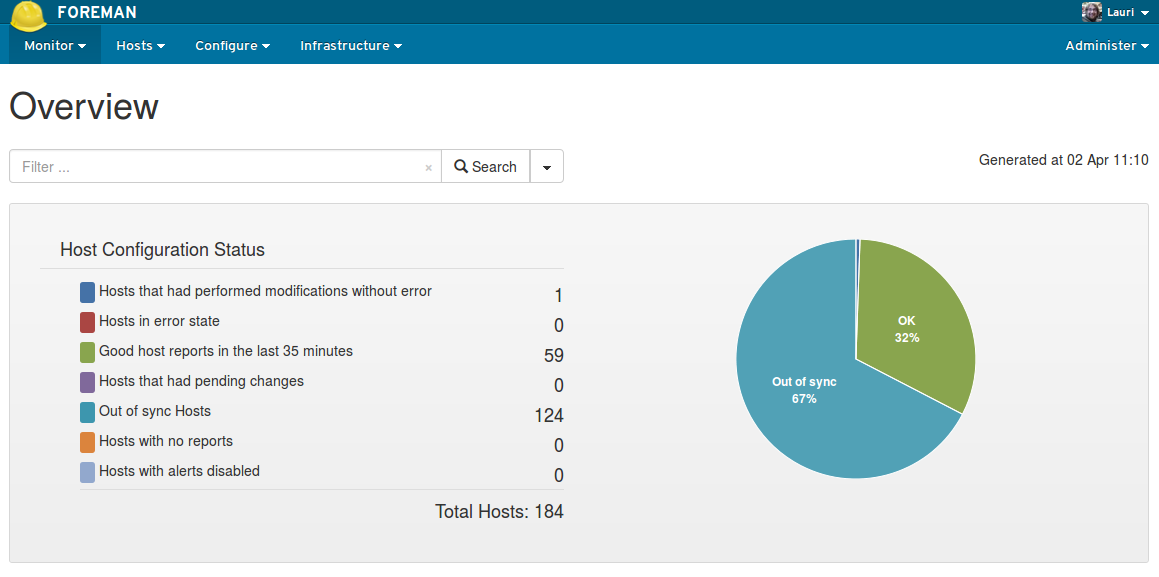
\includegraphics[scale=0.6]{img/foreman.png}}
\caption{Foreman}
\label{fig:digraph}
\end{figure}

Initially OpenLDAP was chosen for authentication and authorization,
but later we switched to Samba4 in order to provide bette
interoperability with Windows workstations.
In fact Samba4 implements Microsoft Active Directory functionality
to large extent,
making it possible to avoid licensing fees while still maintaining
compatibility with Windows workstations wihout
significant work required to configure OpenLDAP and Kerberos to
work in tandem to provide authentication for Windows machines.


\section{Transforming experience into services}

\subsection{Ubuntu deployment service}

As part of the major thesis a more efficient way of deploying Linux-based
workstations was devised.
The resulting software components were used to build an service for
distributing Linux-based operating system templates which can be used to
quickly deploy workstations, laptops and netbooks customized
for particular purpose within 15 minutes over the Internet.
Currently Koodur OÜ mainly maintains template of Ubuntu 14.04 LTS based
workstation which uses lightweight MATE desktop.

\begin{figure}[!htb]
\centering
\scalebox{0.5}{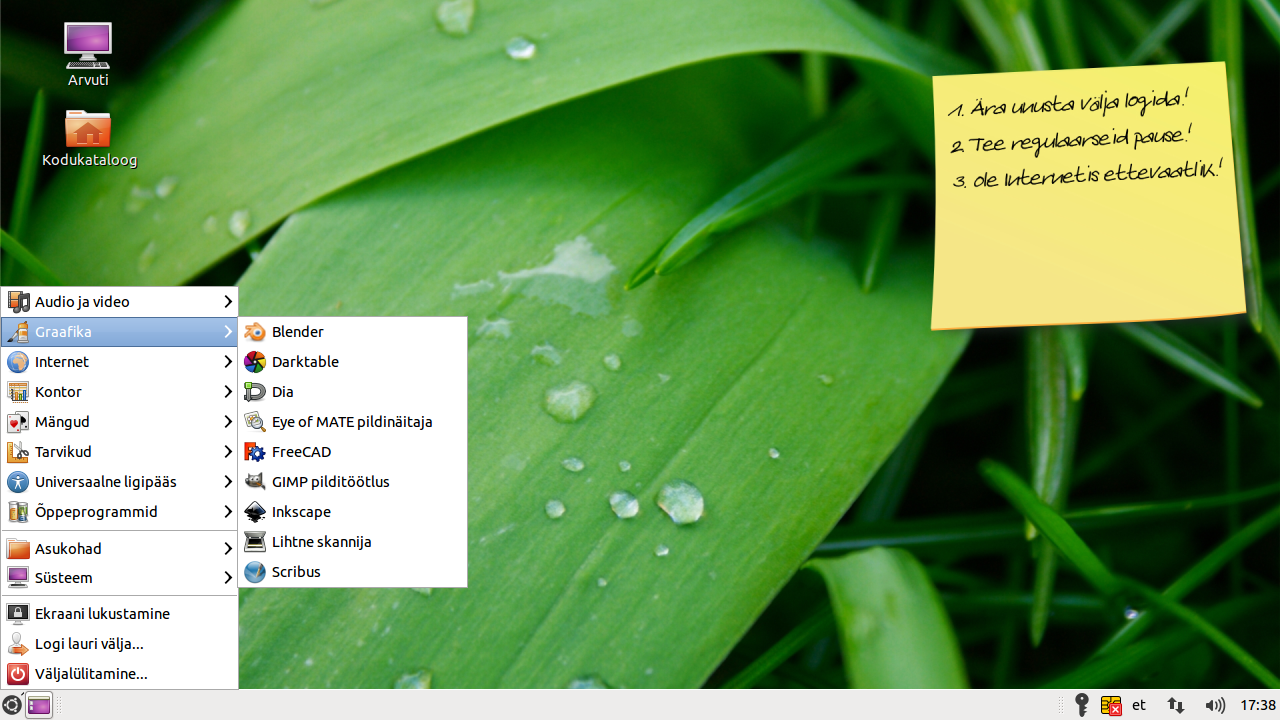
\includegraphics[scale=0.5]{img/edu-workstation}}
\caption{MATE desktop}
\label{fig:digraph}
\end{figure}

We've fine-tuned MATE to slightly mimic Windows XP layout to provide
familiar looks to older generation of users.

\subsection{Software packages}

In addition to Ubuntu software repositories 
we operate an APT repository of 3.6GB which contains
certain proprietary software components necessary
to ease the usage of various hardware equipment.
The repository also contains patched versions of
open-source software which have been modified to cater the
needs of the customers.

\subsection{Remote management}

As the Ubuntu is being continously improved it also requires
continous maintenance of the templates provided by the service.
Running such service also requires extensive knowledge of
how the Linux-based operating system is put together of 
thousands of software components and how they interact with each other.
Occasionally to resolve a problem skills to dive into C code to fix
issues is necessary.

The templates we ship are automatically associated with
the Puppet master instance which lets us manage
the configuration of the machines and apply critical security updates.


\subsection{Identity service}

Our customized Ubuntu 14.04 template integrates
well with existing Active Directory deployments
and Windows file shares.
We also provide Active Directory compatible
authenticationa and authorization service using Samba4.
This service is mainly targeted towards
smaller organizations lacking local
infrastructure and manpower to operate such services.

\subsection{ownCloud}

ownCloud
\footnote{\url{https://owncloud.org/}}
is an open-source project which implements
Dropbox functionality to large extent.
It has German roots and it's distributed under AGPLv3 license.
In conjunction with our authentication service
we provide an ownCloud instance for our customers.

\begin{figure}[!htb]
\centering
\scalebox{0.5}{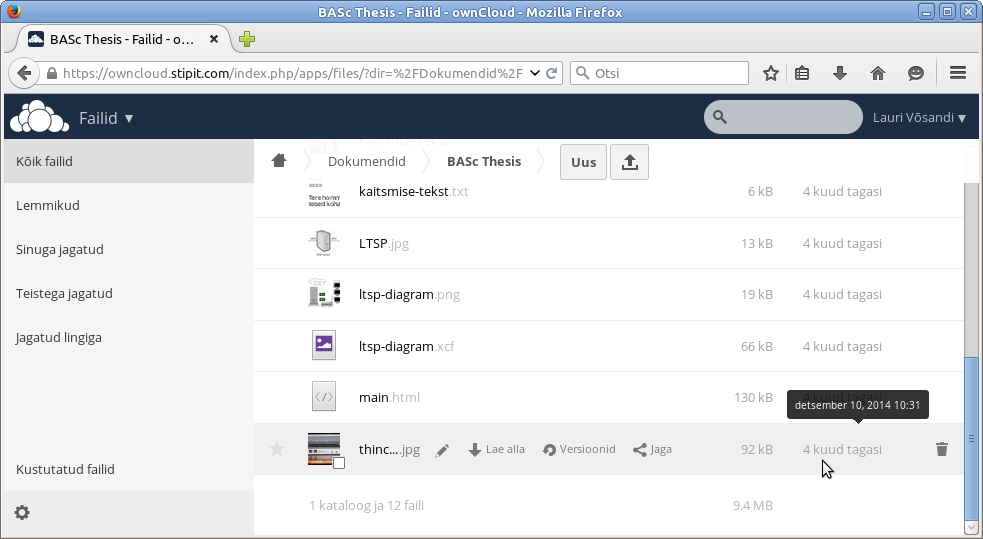
\includegraphics[scale=0.5]{img/owncloud}}
\caption{ownCloud web interface}
\label{fig:digraph}
\end{figure}








\section{Summary}

There is a vast pool of open-source tools available on the Internet
to cater various needs.
Cost to redevelop Linux kernel is estimated to be
approximately \$ 1.4 billion, which is still a fraction
of the development costs of a whole distribution such as Ubuntu
\footnote{\url{
http://www.linuxfoundation.org/sites/main/files/publications/estimatinglinux.html}}.
The components are free for use for businesses, governments and
private use, but attention has to be paid to the license
rights and obligations.

There still is very much confusion regarding open-source licenses
and even recognized brands fail to follow the conditions.
For example in VMware was sued in Germany for failure to comply with GPL
\footnote{\url{https://sfconservancy.org/news/2015/mar/05/vmware-lawsuit/}} in March of 2015.
In the past GPL has proven to be effective in court protecting
the authors of the open-source components.


Snowden revelations pushed various governments to seek for alternatives
to relying on western technology.
For instance use of Windows 8 has been banned in German governmental agencies
\footnote{\url{http://blog.legalsolutions.thomsonreuters.com/law-and-techology/german-government-bans-windows-8-use-nsa-spying-puts-american-companies-risk/}}.
Similariliy Indian Government mandates use of open-source technologies
in order to reduce total cost of ownership and to ensure
strategic control of e-Governance applications and systems
\footnote{\url{http://deity.gov.in/sites/upload_files/dit/files/policy_on_adoption_of_oss.pdf}}.


\section{Conclusion}

There are various political, economic, societal reasons why
companies and governments wish to use open-source software.
Open-source development model cuts costs and due to
it's deduplicative nature it's economically feasible
to pool resources rather
than compete in order to have better service or product in long run.

The educational institutions were used to bootstrap the services and
gain required experience to deliver enterprise grade service and
we have customers popping up in other market segments
and we're expecting the machine count to reach 3000 by the end of 2015.

For developing countries it makes more sense to build
IT infrastructure using open-source components
rather than developing from scratch or licensing proprietary
components from developed countries in order.

Western world, especially countries of post-soviet syndrome
have difficulties fully grasping the whole topic and there's
a lot of misconceptions about open-source and Free Software,
thus awareness raising is necessary.
Estonian Free and Open-Source Software Association
\footnote{\url{http://alvatal.ee/en/}}
is the corresponding body in Estonia and we have a lot of work to do.







\bibliographystyle{plain}
\bibliography{references}

\end{document}
